% V8 research manuscript method draft. Audited against V7 frozen commit
% 061ecf5ddea0a59dcf932b5038ad646b7af454a4. No new performance experiment.
% Citation keys are coordinated with the parent and may be remapped.

\section{面向竞争源判别的双侧镜像嗅觉计算}
\label{sec:m1}

本节研究如何在相同原始观测和有限标定样本下构造源判别表示。Brudner等的双侧嗅觉研究以羽流中心线侧别判断为任务，通过可学习因果时间滤波器、非线性整流和左右镜像相减提取互补线索，并经sigmoid形成侧别预测\ccite{Brudner2026Opponent}。本文保留其前端算子结构，将侧别输出改为竞争源条件下的联合观测分布，并用源对分离目标选择有限通道。镜像滤波、JS散度及贝叶斯归一化均有既有来源；本文拟验证的改造在于三者面向候选源判别的具体组合与选择机制。当前实现采用固定有限核库，尚未实现原母文的自由滤波器学习，也尚未获得优于完整联合观测的原生定位证据。

\subsection{双侧读出、真实时钟与因果镜像算子}

第$t$次同步测量的完整原始块为式\eqref{eq:block}的$X_t$。M1取其浓度与时钟投影$W_t=\{(\tau_{t,n},y_{t,n}^{L},y_{t,n}^{R})\}_{n=1}^{N_t}$，其中$\tau_{t,n}$为严格递增的物理秒值，记$+\equiv L$、$-\equiv R$，分别对应实际配对位置$\mathbf x_{t,n}^{L}$和$\mathbf x_{t,n}^{R}$。通道顺序在训练和测试中固定。原始浓度首先变换为
\begin{equation}
\xi_{t,n}^{\pm}=\log\!\left(1+\frac{[y_{t,n}^{\pm}-b_0]_+}{c_0}\right),\qquad c_0>0,
\label{eq:m1_preprocess}
\end{equation}
其中$[x]_+=\max(x,0)$，背景$b_0$和尺度$c_0$仅由事前配置或训练资料确定。该变换限制大幅值对有限样本估计的影响，但可能丢失低于背景的变化，不能视为无损预处理。

对$N_t>1$，记$\Delta\tau_t=\tau_{t,N_t}-\tau_{t,1}$，采用梯形求积权重
\begin{equation}
\omega_{t,n}=\begin{cases}
(\tau_{t,2}-\tau_{t,1})/(2\Delta\tau_t),&n=1,\\
(\tau_{t,n+1}-\tau_{t,n-1})/(2\Delta\tau_t),&1<n<N_t,\\
(\tau_{t,N_t}-\tau_{t,N_t-1})/(2\Delta\tau_t),&n=N_t.
\end{cases}
\label{eq:m1_time_weights}
\end{equation}
单快照的权重取1。共同强度与静态左右差异分别为
\begin{equation}
e_t=\sum_n\omega_{t,n}\frac{\xi_{t,n}^{+}+\xi_{t,n}^{-}}2,
\qquad
g_t=\sum_n\omega_{t,n}\frac{\xi_{t,n}^{+}-\xi_{t,n}^{-}}2.
\label{eq:m1_even_gradient}
\end{equation}
梯形加权仅实现真实时钟下的时间平均，不能恢复归档中缺失的高频变化。

以$\Xi_t^\pm=(\xi_{t,1}^\pm,\ldots,\xi_{t,N_t}^\pm)^{\mathsf T}$表示变换后序列。母算子的抽象形式是对左右序列施加两个共享时间滤波器，再以相同偏置整流和镜像相减：
\begin{equation}
\begin{aligned}
q_k(\Xi^+,\Xi^-)&=[\langle f_{1k},\Xi^+\rangle+
\langle f_{2k},\Xi^-\rangle+b_k]_+,\\
h_{t,k}&=q_k(\Xi_t^+,\Xi_t^-)-q_k(\Xi_t^-,\Xi_t^+).
\end{aligned}
\label{eq:m1_mirror}
\end{equation}
\begin{figure*}[t]
\centering
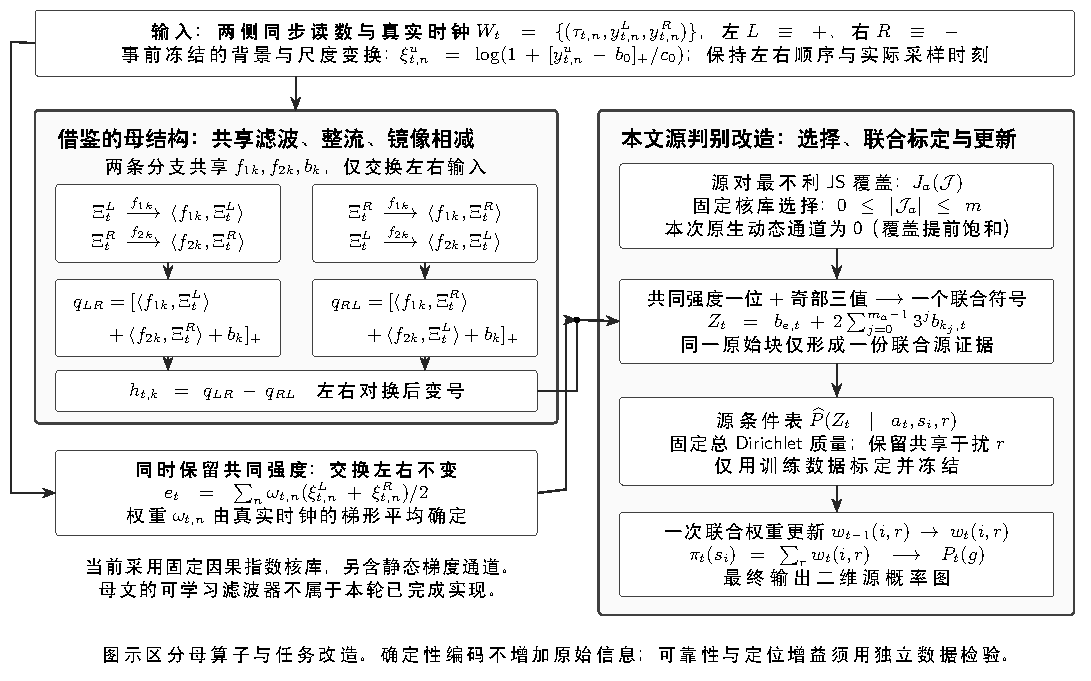
\includegraphics[width=0.98\textwidth]{figures/fig4_mirror.pdf}
\caption{M1的镜像内部运算与源条件证据。两路共享滤波器和偏置，交换左右输入后分别整流，再相减形成反对称响应；共模强度与选中响应只编码为一个联合符号。母算子结构与本文的竞争源选择、联合标定和概率输出分开标识；当前原生选择没有动态镜像通道。}
\label{fig:mirror}
\end{figure*}
式\eqref{eq:m1_mirror}中的滤波、整流和镜像差分属于母方法结构。其反对称性由交换两输入立即得到：$h_k(\Xi^-,\Xi^+)=-h_k(\Xi^+,\Xi^-)$；共同强度$e_t$在交换后不变。这一结构性质不意味着有限训练数据拟合的源条件概率也自动满足空间镜像对称。

当前V7将滤波器限制为因果指数核族\ccite{V7Archive}。设末端时刻$T=\tau_{t,N_t}$，延迟为$\ell_k\ge0$，衰减尺度为$\gamma_k>0$，则
\begin{equation}
\begin{aligned}
w_n^{(\ell_k)}&=
\frac{\mathbf1\{\tau_{t,n}\le T-\ell_k\}
e^{(\tau_{t,n}-T+\ell_k)/\gamma_k}\delta_n}
{\sum_m\mathbf1\{\tau_{t,m}\le T-\ell_k\}
e^{(\tau_{t,m}-T+\ell_k)/\gamma_k}\delta_m},\\
f_{1k}&=w^{(0)}-\eta_k w^{(\ell_k)},\qquad f_{2k}=-w^{(0)},
\end{aligned}
\label{eq:m1_restricted_bank}
\end{equation}
其中$\delta_1=\tau_{t,2}-\tau_{t,1}$，$\delta_n=\tau_{t,n}-\tau_{t,n-1}$（$n\ge2$），$\eta_k$为抑制系数。该离散核与式\eqref{eq:m1_time_weights}采用不同的明示求积规则；历史不支持所需延迟时拒绝计算。核库$\mathcal C$还包含式\eqref{eq:m1_even_gradient}的静态梯度通道。其有限参数、核数和选择规则属于当前实现，不应写成已经学习得到的动物最优滤波器。

传感器响应是输入资格的一部分。式\eqref{eq:sensor}的一阶、无噪声特例可写为$\widetilde y_n^{\pm}=a_n^{\pm}\widetilde y_{n-1}^{\pm}+(1-a_n^{\pm})C_n^{\pm}$，其中$a_n^{\pm}=\exp[-(\tau_n-\tau_{n-1})/\tau_s^{\pm}]$，$C_n^{\pm}$为受体处物理浓度。该关系说明需要标定的响应因素，并非本轮已经执行的真实传感器拟合。两侧响应时间、管路延迟和时钟偏差不相同，可能产生没有空间运动对应的镜像响应。因此，动态分支要求响应标定、同步位置和足够采样带宽；V7另外检查时钟误差与差分传感器延迟之和小于正滞后$\ell_k/3$。该比例是实现门限，不能替代物理带宽校准。

\subsection{源条件联合编码与通道选择}

每个动作$a$在训练数据上冻结共同强度中位数阈值$\theta_{e,a}$和各奇部绝对响应的0.4分位数阈值$\theta_{k,a}$，后者设置数值下限。若选中集合$\mathcal J_a=(k_0,\ldots,k_{m_a-1})$，则一个原始块仅编码为一个联合符号：
\begin{equation}
\begin{aligned}
b_{e,t}&=\mathbf1\{e_t>\theta_{e,a}\},\\
b_{k,t}&=1+\mathbf1\{h_{t,k}>\theta_{k,a}\}
-\mathbf1\{h_{t,k}<-\theta_{k,a}\},\\
Z_t&=b_{e,t}+2\sum_{j=0}^{m_a-1}3^j b_{k_j,t},\qquad O_a=2\cdot3^{m_a}.
\end{aligned}
\label{eq:m1_joint_symbol}
\end{equation}
这里$b_{e,t}$仅保留一位共同强度，不能表述为完整浓度信息得到无损保留。奇部采用关于零对称的三值量化；所有派生量共同进入一个符号，避免把同一块的强度、梯度和镜像响应当成相互独立的多次气体证据。

令$r\in\mathcal R$表示整段共享的有限干扰状态，包括事前声明的释放、传播或响应参数。每个动作、源$s_i$和状态$r$具有$K$个训练块，联合符号计数为$N_{a,i,r}(z)$。采用总质量固定为$\alpha_D>0$的Dirichlet平滑：
\begin{equation}
\widehat P_{\mathcal J}(z\mid a,s_i,r)=
\frac{N_{a,i,r}(z)+\alpha_D/O_a}{K+\alpha_D}.
\label{eq:m1_joint_law}
\end{equation}
不同动作的字母表可补齐到统一张量，但不可到达的补齐符号保持零概率。若保持已有分区不变并新增一个三值通道，则对新增坐标求和恰好返回原估计表，因为$\sum_{b=0}^2\alpha_D/(3O_a)=\alpha_D/O_a$。这排除了通道数增加同时隐式增加平滑总质量的混淆；平滑质量也并不因此获得真实误差概率解释。

通道选择以竞争源对为单位，采用不同干扰状态下的最不利JS距离：
\begin{equation}
\begin{aligned}
d_{ij}(\mathcal J,a)&=\min_{r,r'\in\mathcal R}
\operatorname{JS}\!\big(\widehat P_{\mathcal J}(\cdot\mid a,s_i,r),\\
&\hspace{4.3em}\widehat P_{\mathcal J}(\cdot\mid a,s_j,r')\big),\\
J_a(\mathcal J)&=\sum_{i<j}\min\{d_{ij}(\mathcal J,a),\kappa\}.
\end{aligned}
\label{eq:m1_cover}
\end{equation}
JS散度使用自然对数。以共同强度编码为起点，每轮选择使$J_a$增量最大的未选通道，并在增量不超过$\varepsilon_J$、达到通道上限或全部源对达到阈值$\kappa$时停止。最不利状态比较用于训练目标，不表示在线推断可在每个窗口任意更换固定干扰参数。

\paragraph{算法1（V7源对覆盖标定与在线编码）}
\begin{enumerate}
\item 仅访问训练实现，核验时钟、观测单位、传感器顺序和位置；计算共同强度及核库响应，冻结量化阈值。
\item 对每个动作令$\mathcal J_a=\varnothing$；计算式\eqref{eq:m1_joint_law}--\eqref{eq:m1_cover}。按最大正增量逐项加入通道，并保存每轮增益与停止原因。
\item 冻结动作映射、核库、阈值、联合条件表和训练文件标识。开发数据不参与上述任一步骤。
\item 在线接收新原始块，使用其实际时钟编码式\eqref{eq:m1_joint_symbol}；输出动作编号、唯一块编号及一个$Z_t$，交由共享后验更新一次。
\end{enumerate}

\subsection{联合源推断、信息边界与已发现的退化}

记$w_t(i,r)$为源和共享干扰状态的联合权重。在对应条件观测模型成立时，更新式为
\begin{equation}
\begin{aligned}
w_t(i,r)&=\frac{w_{t-1}(i,r)
\widehat P_t(Z_t\mid a_t,s_i,r,\mathcal F_{t-1})}
{\sum_{j,r'}w_{t-1}(j,r')
\widehat P_t(Z_t\mid a_t,s_j,r',\mathcal F_{t-1})},\\
\pi_t(s_i)&=\sum_r w_t(i,r).
\end{aligned}
\label{eq:m1_posterior}
\end{equation}
二维源图由式\eqref{eq:projection}得到。对共享$r$维持联合权重，避免每次以相同初始先验重新积分干扰状态。当前代码使用固定有限条件表，并主要以驻留块更新工作后验；行进期气体事件另用于M2动作提议。因此，除非进一步建立包含所有已见侧信息的正确条件模型，不能将其称为对完整行进与驻留数据的精确后验。时间窗口不重叠只解决重复使用原始样本的问题，并不自行证明窗口条件独立；重叠窗口必须采用与依赖关系相符的条件增量。

M1遵守式\eqref{eq:dpi}的数据处理边界；从$X_t$提取$W_t$再确定性编码也不会增加信息。可能的改进在于有限样本、模型容量或通信预算下更可靠地估计源判别表示；真正改变可获取观测信息的是下一节的动作选择。固定总平滑且编码分区嵌套时，经验联合JS不小于其边缘JS，因而式\eqref{eq:m1_cover}单调；但特征协同信息可使单个新增通道的增益为零，故不存在一般的次模、贪心全局最优或最小通道数保证。

原生开发实验已经暴露另一种明确退化\ccite{V7Native}：该实验只有两个已标定源，即一个源对；共同强度初始训练JS约为0.242586，已超过$\kappa=0.04$，截断目标随即达到0.04。任何新增通道的目标增量均为零，实际选择集合为空。由此评估的M1只剩共同强度编码，未使用动态镜像通道。此事实说明训练覆盖目标与留出判别目标之间存在落差；不能把相应负结果归因于双机几何已经被独立证伪，也不能通过改写论文将其当作已修复。

对于下一版本，可以研究以源条件预测损失替代硬截断覆盖或学习受因果及镜像约束的核，但这些均属待实现、待前瞻验证的设计。本文不改变已冻结阈值，不追改首轮成绩，也不以“强制加入一个动态通道”作为获得定位收益的证明。未见源的条件预测能力同样尚未由当前有限表建立。

\subsection{计算复杂度与适用条件}

设动作数$N_a$、源数$N_s=|\mathcal S|=J$、干扰状态数$N_r$、核库大小$|\mathcal C|$、代表性块长$N$、最大选中通道数$m$。全部训练特征提取约为$O(N_aN_sN_rK|\mathcal C|N)$；贪心至多评估$N_am|\mathcal C|$个候选集合，每次需要计数并计算$O(N_s^2N_r^2\,2\cdot3^m)$的源对距离。当前限制$m\le3$，仍须面对字母表随通道数指数增长的样本需求。在线实现计算整个核库，复杂度为$O(|\mathcal C|N)$，随后后验更新为$O(N_sN_r)$。上述复杂度不包含原生传播模拟、传感器响应标定和飞行成本。

\section{判别式双机测量与持续反证定位}
\label{sec:m2m3}

M1处理给定窗口中的信息表达，M2与M3共同决定下一窗口的获取方式。M2以气味边界的返回方向生成可执行测量提议，再用竞争源响应差设计双点几何；M3在完整合法源集上分配测量成本，并用独立于旧源赔率的新观测后缀审查当前假设。两模块均已有研究原型\ccite{V7Archive}，但正式原生双无人机主动实验尚未执行\ccite{V7Native}；本节的模型与条件性质不能替代该性能证据。

\subsection{M2：动态边界方向记忆与返回区域}

Siliciano等研究了由气味边界进入、退出事件与运动方向构成的嗅觉导航策略\ccite{Siliciano2026Vector}。本文将方向记忆用于动作候选生成，而不把记忆向量作为第二份源似然。对经过时钟与响应延迟校正的进入事件$k$，令$\widehat{\mathbf d}_k$为真实已观察运动窗口内速度积分后归一化的方向，更新
\begin{equation}
\begin{aligned}
\mathbf m_{k+1}&=a_m\mathbf m_k+b_m\widehat{\mathbf d}_k,\\
\Sigma_{m,k+1}&=a_m^2\Sigma_{m,k}+b_m^2V_k,\qquad
\mathbf u_t=\frac{\mathbf m_t}{\|\mathbf m_t\|}.
\end{aligned}
\label{eq:m2_memory}
\end{equation}
$V_k$包含窗口内方向散布、声明的方向噪声，以及已有有效记忆时新方向与旧记忆单位方向之差的外积项；该递推是忽略跨事件相关项的工程不确定性近似，未被校准为真实协方差。$b_m$不要求等于$1-a_m$。记$k(t)$为截至决策$t$已经完成的合格进入更新次数，后文$\mathbf m_t=\mathbf m_{k(t)}$及$\Sigma_{m,t}=\Sigma_{m,k(t)}$。运动方向来自位置变化及对应段的实际行进方向，不能用机头朝向代替。静止时羽流扫过传感器不建立该运动记忆；方向相消或历史过期时不输出有效返回方向。当前无风版本只更新进入记忆，有风版本增加退出方向和上风门控，仍不等同于母文完整随机运动模型的复现。

现有解析控制演示以两机浓度算术均值大于0.3作为组级气味事件，阈值单位属于该解析后端，并把事件配对到两机位置均值的平面运动。它不等于两机中心处的实测气体，也不证明两机在同一时刻穿越同一物理边界。原生任务中，两侧异步进入、组级事件合成、阈值与响应延迟仍须独立标定；本稿不把这一演示规则写成已经验证的原生边界探测器。

对$\|\mathbf m_t\|>0$，归一化的Jacobian为$J_m=(I-\mathbf u_t\mathbf u_t^\top)/\|\mathbf m_t\|$，方向不确定性矩阵近似为$\Sigma_u=J_m\Sigma_{m,t}J_m^\top$。以当前两机位置均值的平面投影$\bar{\mathbf x}_t\in\mathbb R^2$为原点，取单位法向$\mathbf n_t\perp\mathbf u_t$，定义有限返回区域
\begin{equation}
\begin{aligned}
\mathcal T_t&=\{\bar{\mathbf x}_t+s\mathbf u_t+\zeta\mathbf n_t:\\
&\hspace{2em}0\le s\le L_T,\ |\zeta|\le R_t(s)\},\\
\Sigma_T(s)&=\Sigma_x+q_m\Delta t_m I+(v_{\max}\sigma_\tau)^2I+s^2\Sigma_u,\\
R_t(s)&=r_0+k_T\sqrt{\mathbf n_t^\top\Sigma_T(s)\mathbf n_t}.
\end{aligned}
\label{eq:m2_tube}
\end{equation}
其中$\Delta t_m$是记忆物理年龄，$q_m$为位置漂移方差率，$\sigma_\tau$为延迟不确定度。该区域是工程不确定性传播结果，尚未校准为某个概率覆盖水平。它随当前位置平移，保留相对返回方向，不把上次边界坐标当成静止目标；也不承担源概率更新或安全航路认证。

\subsection{M2：面向竞争源响应差的双点几何}

当前几何接口在共同测量高度上设计平面中心$\mathbf q$、间距$d$和单位基线方向$\mathbf u$，两测点为$\mathbf q\pm d\mathbf u/2$。三维位置仍由任务数据合同记录，但本文不将该平面接口扩写成已实现的一般三维编队控制。由训练实现或在线因果可得模型提供源$s_i$的原始有限窗均值$\mu_i(\mathbf q)$、空间梯度$\nabla\mu_i(\mathbf q)$和偶奇联合协方差$\Sigma_i(a)$。这些量不读取未观测测试全场；其原始浓度尺度与M1的对数编码分开。

在合法局部半径内，一阶双点响应预测为
\begin{equation}
\bar{\mathbf z}_i(a)=
\begin{bmatrix}\mu_i(\mathbf q)\\
\frac d2\mathbf u^\top\nabla\mu_i(\mathbf q)\end{bmatrix},
\quad
\Delta\mathbf z_{ij}(a)=\bar{\mathbf z}_i(a)-\bar{\mathbf z}_j(a),
\label{eq:m2_response}
\end{equation}
并以完整联合协方差形成设计距离
\begin{equation}
D_{ij}^{\mathrm{geom}}(a)=
\Delta\mathbf z_{ij}^{\top}
[\Sigma_i(a)+\Sigma_j(a)+\lambda_gI]^{-1}
\Delta\mathbf z_{ij}.
\label{eq:m2_geometry_score}
\end{equation}
$\lambda_g\ge0$为事前声明的正则量，不能利用开发结果反复调节。池化矩阵必须正定；当前代码在不满足时拒绝输入，要求提供合格方差或明确正则量，不静默使用伪逆。式\eqref{eq:m2_geometry_score}不是气体似然、KL散度或审计统计量；协方差的交叉项只使用一次。当前训练接口采用普通RBF拟合均值及解析梯度，该适配本身不作为新算法贡献，且外推与协方差池化仍需独立校准。

上述几何有明确适用边界。若局部Hessian范数有界$\|\nabla^2\mu_i\|\le M_i$，双点精确偶部与$\mu_i(\mathbf q)$、精确奇部与一阶梯度项的误差均不超过$M_id^2/8$。这由两端Taylor余项相加、相减得到；当前接口检查局部半径，却没有实测证明$M_i$界。长基线应采用精确端点预测，不能借短基线展开赋予其资格。当两源均值相等、联合协方差不随方向变化且梯度差$\Delta\mathbf g\ne0$时，式\eqref{eq:m2_geometry_score}由$\mathbf u=\pm\Delta\mathbf g/\|\Delta\mathbf g\|$最大化；梯度差为零时各方向并列。方向相关噪声、成本及可达性存在时须共同比较。

当前M1的阈值与联合条件表按有限动作编号标定，因此M2实际执行的动作须落在事前安装集合$\mathcal A^{\rm inst}$内，并与其位置、传感器、时钟及读出定义一致。RBF可计算新几何的均值和梯度提议，但不会自动为新动作生成合格的M1联合似然。未安装的中心、基线或方向仍需独立动作标定及冻结，或经验证的参数化条件预测接口；当前原型没有自动完成这一步。

M2枚举已安装且通过端点合法性、间距和线性化半径检查的动作，输出全部动作与源对的设计距离矩阵。记当时合法且剩余预算可负担的集合为$\mathcal A_t^{\rm legal,aff}\subseteq\mathcal A^{\rm inst}$，M2利用掩码形成$\mathcal A_t^{\rm use}\subseteq\mathcal A_t^{\rm legal,aff}$。返回区域内存在超过判别阈值的动作时，优先提出这些动作；否则开放区域外的合法复测。某个均值型距离为零不代表完整观测分布不可区分，高阶结构和协方差差异仍可能有用。返回区域及利用掩码不能禁止M3在$\mathcal A_t^{\rm legal,aff}$内的覆盖和显式挑战。现有代码的端点检查也不自动证明整段航路无碰撞或两机同步到达。

\subsection{M3：完整源集上的成本分配与持续覆盖}

\begin{figure*}[t]
\centering
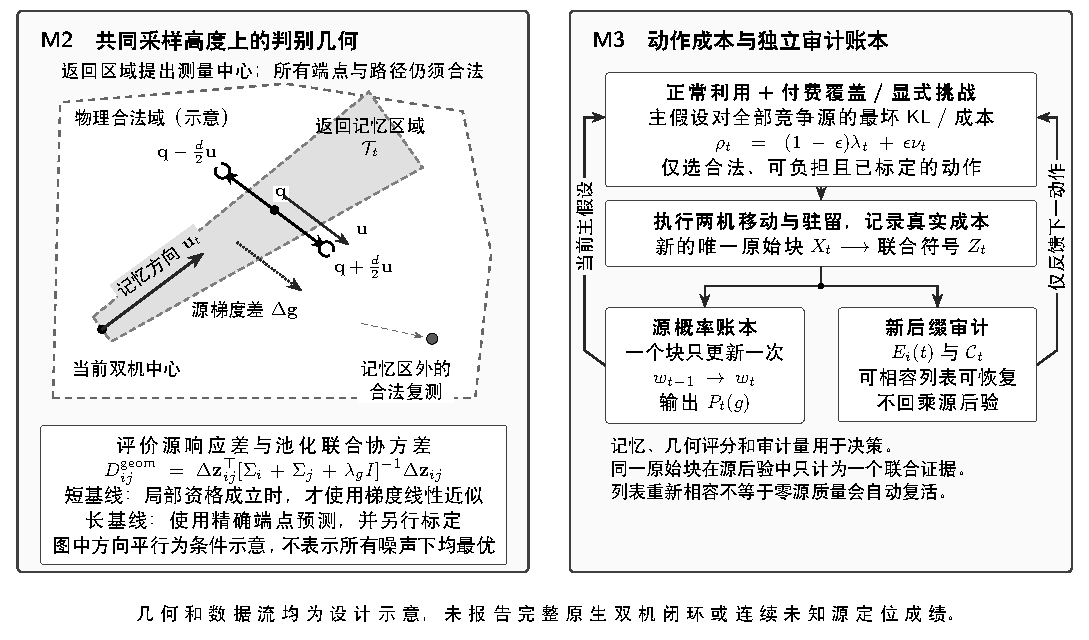
\includegraphics[width=0.98\textwidth]{figures/fig5_geometry_audit.pdf}
\caption{双机判别几何与持续反证决策示意。左侧为共同高度下的返回区域、中心与双点基线，响应差分数仅用于动作设计；返回区域外的合法测量仍可被覆盖或挑战。右侧为新观测进入一次后验更新与独立后缀审计，审计只反馈下一动作。全部动作须具备相同编号下已标定的条件预测，几何示意不是原生飞行验证。}
\label{fig:geometry}
\end{figure*}

主动序贯假设检验提供了按竞争假设差异分配测量的理论基础\ccite{Hsu2025Tradeoffs}，非同质成本研究进一步区分测量次数与资源消耗\ccite{Vershinin2026Costs}。本文沿用这些目标结构，研究其与低后验候选持续复核、M2区域外挑战和新后缀审计的结合，不将KL、线性规划或Chernoff原则本身列为原创。

给定当前最大工作后验源$i_t=\arg\max_i\pi_{t-1}(s_i)$，先从联合权重得到用于规划的干扰条件权重
\begin{equation}
\begin{aligned}
\beta_{ir,t}&=\begin{cases}
w_{t-1}(i,r)/\pi_{t-1}(s_i),&\pi_{t-1}(s_i)>0,\\
\beta_{ir,0},&\pi_{t-1}(s_i)=0,
\end{cases}\\
p_{i,t}^{a}(z)&=\sum_r\beta_{ir,t}\widehat P(z\mid a,s_i,r).
\end{aligned}
\label{eq:m3_predictive}
\end{equation}
其中$\beta_{ir,0}$为安装模型对源$s_i$的归一干扰先验。零源质量时退回该先验，只用于提出反事实测量，不给工作后验补回源质量。当前程序中的$\widehat P$是冻结有限表；此处预测不因此成为对全部行进历史的真实条件律。源对分离及动作成本定义为
\begin{equation}
D_{ij,t}(a)=\sum_zp_{i,t}^a(z)\log\frac{p_{i,t}^a(z)}{p_{j,t}^a(z)},\qquad c_t(a)>0.
\label{eq:m3_kl}
\end{equation}
$c_t(a)$应包括到位、恢复、稳定和同步采样的完整成本。由安装表计算的KL属于模型内设计量，不能当作真实未知羽流信息率的校准下界。以所有$j\ne i_t$为对手，在非空利用域$\mathcal A_t^{\rm use}$上求
\begin{equation}
\max_{\lambda\in\Delta(\mathcal A_t^{\rm use})}
\frac{\min_{j\ne i_t}\sum_a\lambda_aD_{i_tj,t}(a)}
{\sum_a\lambda_ac_t(a)}.
\label{eq:m3_cost_ratio}
\end{equation}
本式及下式的动作求和均在$\mathcal A_t^{\rm use}$内。令$y_a=\lambda_a/(\sum_b\lambda_bc_t(b))$，可等价转为
\begin{equation}
\begin{aligned}
\max_{y\ge0,v}\quad&v,\\
\mathrm{s.t.}\quad&\sum_ac_t(a)y_a=1,\\
&\sum_ay_aD_{i_tj,t}(a)\ge v,\quad j\ne i_t;\\
&\lambda_a=\frac{y_a}{\sum_by_b}.
\end{aligned}
\label{eq:m3_lp}
\end{equation}
由$\lambda$到$y$及反向归一化均保持式\eqref{eq:m3_cost_ratio}的值，给出等价性。求解后以零概率延拓到$\mathcal A_t^{\rm legal,aff}$。实现内部可用资源份额$c_t(a)y_a$求解，但抽样频率必须按$y$归一化，不能直接使用资源份额。两源情形只有一个对手约束，退化为选择最大$D/c$的动作，因此两源固定探针实验不能验证多候选分配机制。

为使低后验源仍有机会得到反证性测量，执行分布定义为
\begin{equation}
\rho_t(a)=(1-\epsilon)\lambda_t(a)+\epsilon\nu_t(a),
\qquad 0<\epsilon\le1,
\label{eq:m3_coverage}
\end{equation}
其中$\nu_t$在$\mathcal A_t^{\rm legal,aff}$上预先定义，并与源后验无关；完整版默认取均匀正覆盖。若该集合为空，则结束当前预算内采样，不再求分配或生成观测。M2仅限制正常利用分配，覆盖及显式挑战可访问利用域外的合法可负担动作。当最坏信息率未超过事前数值容差、利用域为空、支持不匹配造成无限KL或审计指定挑战源$j$时，当前原型转用$\min\{D_{i_tj,t}(a),D_{ji_t,t}(a)\}/c_t(a)$在$\mathcal A_t^{\rm legal,aff}$上选择源对挑战，仍保留覆盖分量。无显式挑战时，程序在具有正双向分离的对手间轮转；若不存在，则在全部对手间轮转。若所选源对的最佳分数仍未超过容差，利用分布也设为$\nu_t$，最终$\rho_t=\nu_t$。这些回退是明示工程规则，不继承完整线性规划最优性。

在固定合法动作域上，若$\nu(a)>0$且连续执行$T$步，则由每步条件概率下界可得
\begin{equation}
\Pr\{N_a(T)=0\}\le[1-\epsilon\nu(a)]^T.
\label{eq:m3_coverage_bound}
\end{equation}
该界说明错误后验不会关闭动作$a$的访问概率；它不证明动作可辨、有限预算必然恢复或估计KL准确。预算尾段动作被移除时，应报告实际可负担集合，不能延用固定全域的无限期保证。覆盖每步的期望成本为$\epsilon\sum_a\nu_t(a)c_t(a)$，并非免费探索。

\subsection{M3：新后缀审计与可恢复候选列表}

旧观测可能形成错误高置信，因而审计从只依赖已见信息的时刻$t_0$开始，所有源--干扰状态的后缀似然初始化为1，不继承旧源赔率。可预测替代分布与复合零假设最大似然的结构已有统计学基础\ccite{Wasserman2020Universal}，近期量子序贯检验给出其另一领域应用\ccite{Zecchin2025QSUT}。这里仅借鉴已读取作者稿中的统计结构，不涉及量子硬件，也不将其量子任务实验当作气源定位验证。

对固定共享状态$r$定义
\begin{equation}
\begin{aligned}
L_{ir}(t)&=\prod_{k=t_0+1}^{t}
P_k(Z_k\mid s_i,r,a_k,\mathcal F_{k-1}),\\
Q_{-i}(t)&=\sum_{j\ne i,r}w_{jr}^{(-i)}L_{jr}(t),
\end{aligned}
\label{eq:m3_suffix}
\end{equation}
其中$w_{jr}^{(-i)}>0$在审计前固定、对$j\ne i,r$归一化。当$Q_{-i}(t-1)>0$时，由后缀混合得到下一结果出现前冻结的替代预测
\begin{equation}
\begin{aligned}
q_{-i,t}(z)&=\sum_{j\ne i,r}
\frac{w_{jr}^{(-i)}L_{jr}(t-1)}{Q_{-i}(t-1)}\\
&\hspace{3em}\cdot P_t(z\mid s_j,r,a_t,\mathcal F_{t-1}),\\
E_i(t)&=\frac{Q_{-i}(t)}{\max_rL_{ir}(t)}.
\end{aligned}
\label{eq:m3_evalue}
\end{equation}
分母对整段相同$r$的似然取最大值，不能改为逐时刻分别取最大后相乘。若$Q_{-i}(t-1)=0$，下一步可选择任意非负且和为1的替代预测，当前程序取字母表上的均匀分布；但累计替代路径质量继续保持零，不因重新归一化而复活。所有安装状态均不能解释整个后缀时，报告模型支持失败，不以人为概率下限产生一个认证赢家。对模型概率统一添加下限会改变零假设族和检验律，必须重新校准，不能声称原风险结论无条件保留。

\paragraph{条件性质（模型内真源覆盖）}
若真源$s_i$和一个固定真干扰状态$r_*$均在安装族中；$P_k$是给定同一实际过去及动作的真实正规条件律；动作、审计起点和替代预测仅使用过去；且原始观测不被重复当作新条件增量，则
\begin{equation}
\Pr_{s_i,r_*}\{\exists t\ge t_0:E_i(t)\ge1/\alpha_A\}\le\alpha_A.
\label{eq:m3_risk}
\end{equation}
证明如下：$\max_rL_{ir}\ge L_{ir_*}$，故$E_i\le M_t=Q_{-i}/L_{ir_*}$。正规可预测的替代分布使$M_t$为非负检验超鞅；在共同支持上，每步似然比的条件期望不超过1。由Ville不等式得到$M_t$的越界概率界，点态支配再得到式\eqref{eq:m3_risk}。$E_i$自身不必为超鞅。该性质是对标准似然比工具在当前有限族中的适配证明，不是新发明的概率不等式。

训练拟合的直方图或Gaussian并不自动满足真实条件族包含性；当前审计只有模型内解释。即使拟合算法在每次观测前冻结，也仍需独立证明校准和时间依赖处理；仅有可预测性并不足以获得物理风险保证。多个审计重复启动还须分配累计错误预算。原生环境中的传感器失配、未见风场与连续干扰状态覆盖均待验证。

当前可相容集与从未越界集分别为
\begin{equation}
\begin{aligned}
\mathcal C_t&=\{s_i:E_i(t)<1/\alpha_A\},\\
\mathcal C_t^{\mathrm{ever}}&=
\{s_i:\max_{t_0\le u\le t}E_i(u)<1/\alpha_A\}.
\end{aligned}
\label{eq:m3_lists}
\end{equation}
前者允许重新进入，后者单调缩小；二者都不是源概率分布。若当前最大后验源不在$\mathcal C_t$，原型从仍相容的替代源中选择审计量最小者作为下一次显式挑战。此反馈只改变动作提议，不修改旧源概率，不将$E_i$或其倒数重新乘入式\eqref{eq:m1_posterior}。因此，同一原始块可以分别用于后验计算和决策审查，但在源后验中只计入一次。所有源仍须保留于合法候选支撑；初始质量为零或已由结构零永久消去的源不能靠乘法更新恢复。

\subsection{模块接口、伪代码与区别于普通信息增益的作用}

普通期望信息增益根据后验加权的平均熵下降选择动作；M2提供由方向记忆和响应差生成的几何提议，M3正常分配关注当前主假设对全部竞争源的最坏单位成本分离，并额外保留后验独立覆盖及审计触发的源对挑战。目标不同不意味着后者必然更优；必须在相同两机资源、相同原始信息权限和完整实际成本下与联合EIG比较。当前控制实现的行进信息仅进入M2，这一额外信息通道必须同时提供给强基线或单独消融。

\paragraph{算法2（统一测量与源概率更新）}
\begin{enumerate}
\item 初始化严格正的源先验$\pi_0$、归一干扰先验$\beta_{ir,0}$与联合权重$w_0(i,r)=\pi_0(s_i)\beta_{ir,0}$；冻结已安装动作、M1模型、传感器资格、资源预算及最大步数。初始化方向记忆与观测账本，指定单次审计错误预算$\alpha_A$，从$L_{ir}=Q_{-i}=1$启动审计。当前演示仅用一个账本；若另行设计重复启动，须事前分配累计错误预算。
\item 每轮根据已发生的运动与气味事件更新M2记忆，在已安装动作中构造利用域及合法可负担域。预算耗尽、达到预设步数或合法可负担域为空时结束循环。
\item 由当前联合权重计算源预测，针对全部合法源在利用域求成本分配，并在合法可负担域叠加付费覆盖；若旧主假设受到新后缀反证，则指定源对挑战。按明示回退规则处理空利用域及无正分离情形，并抽取下一动作。
\item 在新结果出现前冻结审计预测，执行移动、稳定与采样，记录两机位置、原始时钟、传感器标识、实际成本和唯一块编号。观测资格或时序核查失败时停止并报告原因，不插补新证据。
\item 调用M1产生一个联合符号，更新一次源--干扰权重并输出二维源图；在独立审计账本更新后缀似然和候选列表。若全部安装状态不支持观测或审计后缀，停止并报告模型支持失败，不据此认证某个源。
\item 核算实际资源消耗，将审计反馈用于下一动作后返回步骤2；派生记忆、规划分数和审计量不作为额外气体似然。结束时保存最后有效源图和诊断。审计列表只剩一个源不触发自动成功，也不等同于真实位置已经正确。
\end{enumerate}

若中心、间距、方向个数分别为$N_q,N_d,N_u$，M2几何评分约为$O(N_qN_dN_uN_s^2)$；当前方向历史采用列表保存和扫描，不能将整段实现宣称为常数时间。令$O=\max_a O_a$为统一补齐后的联合字母表大小，M3完整源对KL计算为$O(N_aN_s^2O)$，之后还需有限线性规划求解；审计预测混合约为$O(N_s^2N_rO)$，一次观测更新约为$O(N_sN_r)$。原型固定动作成本和返回共同起点的演示尚不覆盖一般时变航路成本；正式双机实验须统一规划成本、执行时间及审计记账，并独立验证路径和同步到达。
